\documentclass[12pt, a4paper]{article}
\usepackage{graphicx}
\usepackage{tikz}
\usetikzlibrary{shapes.geometric, arrows}

\title{Sprawozadanie lernicng}
\author{Tymon Łazowy}
\date{123,2123,12}


\tikzstyle{startstop} = [ellipse, rounded corners, minimum width=2cm, minimum height=1cm,text centered, draw=black, 
fill=red!0]

\tikzstyle{io} = [trapezium, 
trapezium stretches=true, % A later addition
trapezium left angle=70, 
trapezium right angle=110,
text width=2cm,
minimum width=2cm, 
minimum height=1cm, text centered, 
draw=black, fill=blue!0]

\tikzstyle{process} = [rectangle, 
minimum width=2cm, 
minimum height=1cm, 
text centered, 
text width=2cm, 
draw=black, 
fill=orange!0]

\tikzstyle{decision} = [diamond, 
minimum width=1cm, 
minimum height=1cm, 
text centered, 
draw=black, 
fill=green!0]
\tikzstyle{arrow} = [thick,->,>=stealth]
\begin{document}

\begin{figure}
    \centering  
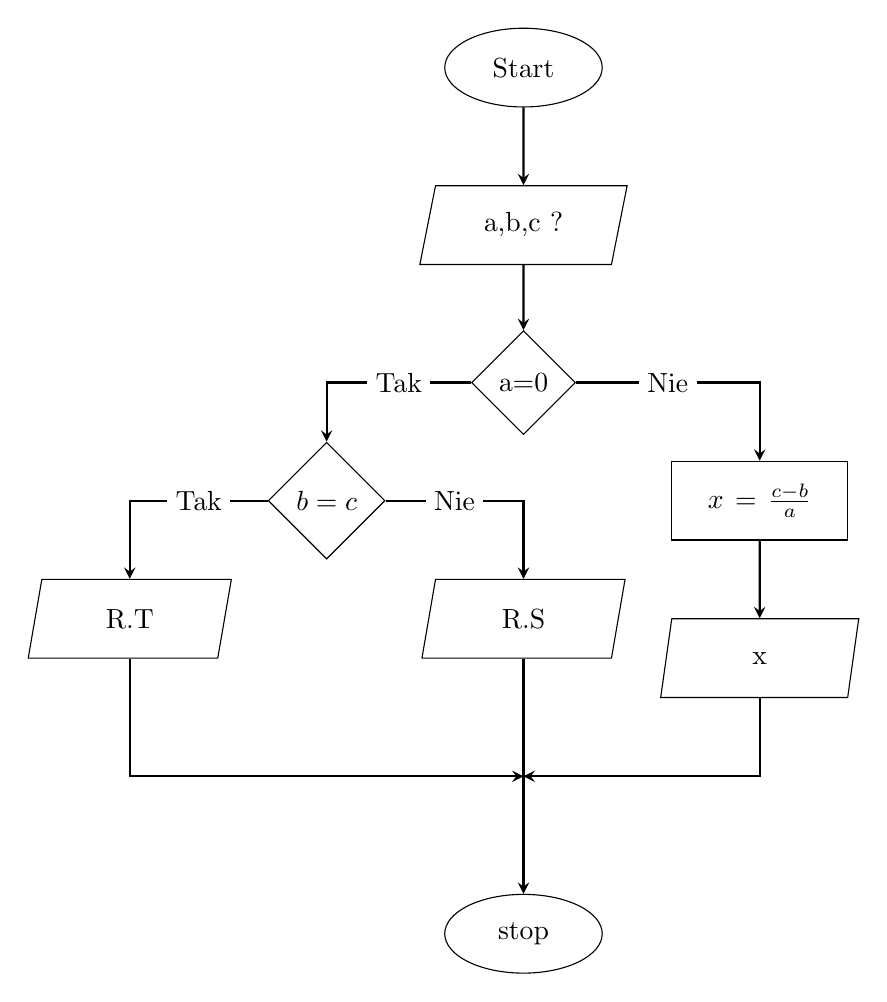
\begin{tikzpicture}[node distance=2cm]

\node (start) [startstop] {Start};
\node (in1) [io, below of=start] {a,b,c ?};
\node (dec1) [decision, below of=in1] {a=0};
\node (pro1) [process, right of=dec1, xshift=1cm, yshift=-1.5cm] {$x=\frac{c-b}{a}$};
\node (in4) [io, below of =pro1]{x};
\node (dec2) [decision, left of=dec1, xshift=-0.50cm, yshift=-1.5cm] {$b=c$};
\node (in2) [io, right of=dec2, xshift=0.50cm, yshift=-1.5cm] {R.S};
\node (in3) [io, left of=dec2, xshift=-0.50cm, yshift=-1.5cm] {R.T};
\node (meeting)[coordinate,below of =in2]{};
\node (stop) [startstop, below of =meeting, yshift=0]{stop};

\draw [arrow] (start) -- (in1);
\draw [arrow] (in1) -- (dec1);
%\draw [arrow] (dec1) -| node[anchor=south west] {yes} (dec2);
\draw[arrow] (dec1) -| (dec2) node[pos=0.25,fill=white,inner sep=3]{Tak};
\draw[arrow] (dec1) -| (pro1) node[pos=0.25,fill=white,inner sep=3]{Nie};
\draw[arrow] (dec2) -| (in3) node[pos=0.25,fill=white,inner sep=3]{Tak};
\draw[arrow] (dec2) -| (in2) node[pos=0.25,fill=white,inner sep=3]{Nie};
\draw [arrow] (pro1) -- (in4);   
\draw [arrow] (in4) |- (meeting);
\draw [thick] (in2) |- (meeting);
\draw [arrow] (in3) |- (meeting);
\draw [arrow] (meeting)--(stop);

\end{tikzpicture}

    \caption{Funkcja liniowa}
    \label{flow1}
\end{figure}
\end{document}

